נתונות $n$ משימות 
$A = \{a_1, \ldots, a_n\}$
נסמן ב-%
$t(a_i)$
את הזמן הנדרש לביצוע משימה 
$a_i$
וב-%
$d(a_i)$
את זמן הסיום הרצוי של המשימה.
בהינתן סדר ביצוע המשימות (פרמוטציה)
$\pi:A \to [n]$.
נסמן ב-%
$\delta(a_i)$
את זמן הסיום של המשימה 
$a_i$,
כלומר
$$\delta(a_i) = \sum_{i \leq \pi(a_i)} t(\pi^{-1}(i))$$
נסמן ב-%
$l(a_i) \defeq \delta(a_i) - d(a_i)$
את האיחור בביצוע משימה 
$a_i$.
רוצים למצוא סדר שממזער את האיחור המקסימלי, כלומר
$$
\text{arg}\min_\pi \{\max_i l(a_i)\}
$$

\textbf{דוגמה:}
בהינתן שלוש המשימות הבאות:
\begin{english}
\begin{center}
\begin{tabular}{|l|l|l|}
\hline
A & t & d
\\
\hline
$a_1$ & 2 & 7
\\ \hline
$a_2$ & 3 & 10
\\ \hline
$a_3$ & 5 & 5
\\ \hline
\end{tabular}
\end{center}
\end{english}

שני שיבוצים אפשריים, אחד ללא איחור כלל והשני עם איחור של 5.

\begin{center}
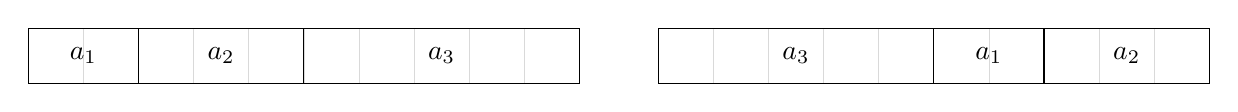
\begin{tikzpicture}[x=7mm, y=7mm]
\draw[very thin, gray!30] (0,0) grid[step=7mm] (10,1);
\draw (0,0) rectangle +(2,1) node[pos=.5] {$a_1$};
\draw (2,0) rectangle +(3,1) node[pos=.5] {$a_2$};
\draw (5,0) rectangle +(5,1) node[pos=.5] {$a_3$};

\begin{scope}[xshift=8cm]
\draw[very thin, gray!30] (0,0) grid[step=7mm] (10,1);
\draw (0,0) rectangle +(5,1) node[pos=.5] {$a_3$};
\draw (5,0) rectangle +(2,1) node[pos=.5] {$a_1$};
\draw (7,0) rectangle +(3,1) node[pos=.5] {$a_2$};
\end{scope}
\end{tikzpicture}
\end{center}


האלגוריתם החמדן יבצע את המשימות בסדר לא יורד של זמני הסיום הרצויים.

\textbf{הוכחת נכונות}

נוכיח באינדוקציה את הטענה הבאה:

לכל $i$ קיים פתרון אופטימלי שמבצע את $i$ המשימות הראשונות לפי זמני הסיום שלהן.

בסיס: טריוויאלי

צעד: נסתכל על המשימה, $a$, שזמן הסיום שלה הוא ה-%
$i+1$
לפי סדר לא יורד. 
אם הפתרון האופטימלי מבצע את המשימה הזאת בזמן 
$i + 1$
סיימנו, אחרת הוא מבצע אותה בזמן 
$j > i + 1$
נסתכל על סדר ביצוע המשימות מזמן 
$i + 1$
עד זמן 
$j$:
$$
b_{i + 1}, \ldots, b_{j - 1}, a
$$

נבחן פתרון שמבצע את המשימות הללו בסדר הבא:

$$
a, b_{i + 1}, \ldots, b_{j - 1}
$$

נבדוק את האיחור המקסימלי של משימות אלו (האיחור המקסימלי של יתר המשימות לא השתנה) 
ונניח בשלילה שהוא גדל (אחרת סיימנו). 
אם זמן הסיום גדל זה חייב להיות בגלל אחת מהמשימות 
$b_{i+1}, \ldots, b_{j - 1}$,
נסמן אותה ב-$b$. נסמן את זמן הסיום שלה לפי הסדר החדש ב-%
$\delta'(b)$
אנחנו יודעים אבל ש-%
$\delta'(b) \leq \delta(a)$
וגם ש-%
$d(a) \leq d(b)$
ולכן
$\delta'(b) - d(b) \leq \delta(a) - d(a)$.

